\documentclass{beamer}
\usetheme{Madrid}
\usepackage[T1]{fontenc}
\usepackage{mathpazo}
\usepackage{graphicx}
\usepackage{booktabs}
\usepackage{tikz}
\usetikzlibrary{positioning,arrows.meta,shapes.geometric,fit,backgrounds,calc}
\definecolor{cetnavy}{RGB}{10,26,63}
\definecolor{cetlight}{RGB}{225,231,242}
\setbeamercolor{structure}{fg=cetnavy}
\setbeamercolor{frametitle}{bg=cetnavy,fg=white}
\setbeamercolor{title}{bg=cetnavy,fg=white}
\setbeamertemplate{navigation symbols}{}
% =====================================================================
%  EDIT YOUR DETAILS HERE — this ONE file feeds every abstract & deck.
%  (Change a value, recompile; all 36 documents update.)
% =====================================================================
\newcommand{\seminarName}{Aflah Muhammed P}      % <-- your full name (guessed from your email; please verify)
\newcommand{\seminarRoll}{TVE00CS000}            % <-- your university register/roll number
\newcommand{\seminarClassRoll}{00}               % <-- your class roll no (the short one)
\newcommand{\seminarGuide}{Prof.\ <Guide Name>}  % <-- your guide
\newcommand{\seminarDept}{Department of Computer Science and Engineering}
\newcommand{\seminarCollege}{College of Engineering Trivandrum}
\newcommand{\seminarShortCollege}{CET}           % shown in the slide footer, e.g. "Aflah Muhammed P (CET)"
\newcommand{\seminarShortTitle}{B.Tech Seminar}  % middle of the slide footer
\newcommand{\seminarDate}{July 31, 2026}
% ---------------------------------------------------------------------
% Optional: put a logo image named  cet_logo.png  in this folder and it
% will appear on every title slide automatically. If absent, it is skipped.
% =====================================================================

\title[\seminarShortTitle]{SWE-smith: Scaling Data for Software-Engineering Agents}
\author[\seminarName\ (\seminarShortCollege)]{\seminarName \\ \seminarRoll \\ Roll No: \seminarClassRoll \\ Guide: \seminarGuide}
\institute[\seminarShortCollege]{\seminarDept \\ \seminarCollege}
\date{\seminarDate}
\titlegraphic{\IfFileExists{cet_logo.png}{\includegraphics[height=1.1cm]{cet_logo.png}}{}}
\begin{document}
\begin{frame}\titlepage\end{frame}
\begin{frame}{Table of Contents}\tableofcontents\end{frame}
\section{Introduction}
\begin{frame}{Agents that fix code}
\begin{itemize}
\item LM agents now resolve real GitHub issues.
\item Progress is bottlenecked by scarce training data.
\item SWE-smith: an automated factory for bug-fix tasks.
\item Turns any Python repo into verified tasks.
\item About 50{,}000 instances from 128 repositories.
\end{itemize}
\end{frame}

\section{Literature Survey}
\begin{frame}{Prior data and agents}
\textbf{\textit{Where the data came from}}
\begin{itemize}
\item SWE-bench: tasks mined from real pull requests.
\item SWE-agent: agent-computer interface over a repo.
\item Earlier open sets held only thousands of instances.
\item Real-PR mining is slow and storage-heavy.
\item Motivates scalable, synthetic task generation.
\end{itemize}
\end{frame}

\section{Motivation}
\begin{frame}{Why scale the data}
\begin{itemize}
\item Open agents lag proprietary coding models.
\item Each task needs a reproducible environment.
\item Prior pipelines needed tens to hundreds of TBs.
\item Few open instances limit fine-tuning.
\item Need cheap, verifiable task supply.
\end{itemize}
\end{frame}

\section{Problem Statement}
\begin{frame}{The precise problem}
\begin{itemize}
\item Produce many verifiable bug-fix tasks.
\item Without hand-mining GitHub pull requests.
\item Each task needs an objective pass/fail signal.
\item Keep storage and setup cost low.
\item Scale to arbitrary Python repositories.
\end{itemize}
\end{frame}

\section{Objectives}
\begin{frame}{Goals and contributions}
\begin{itemize}
\item Automated pipeline for any Python repo.
\item Diverse strategies to synthesize bugs.
\item Self-labeled, execution-verified fixes.
\item Large open dataset plus a trained agent.
\item New state of the art among open models.
\end{itemize}
\end{frame}

\section{Methodology Overview}
\begin{frame}{Core idea: a self-labeling factory}
\begin{itemize}
\item Start from a working repo and its tests.
\item Inject a bug so passing tests now fail.
\item Original code plus tests is the gold fix.
\item An LM writes a realistic issue description.
\end{itemize}
\end{frame}
\begin{frame}{Methodology Overview}
\begin{center}
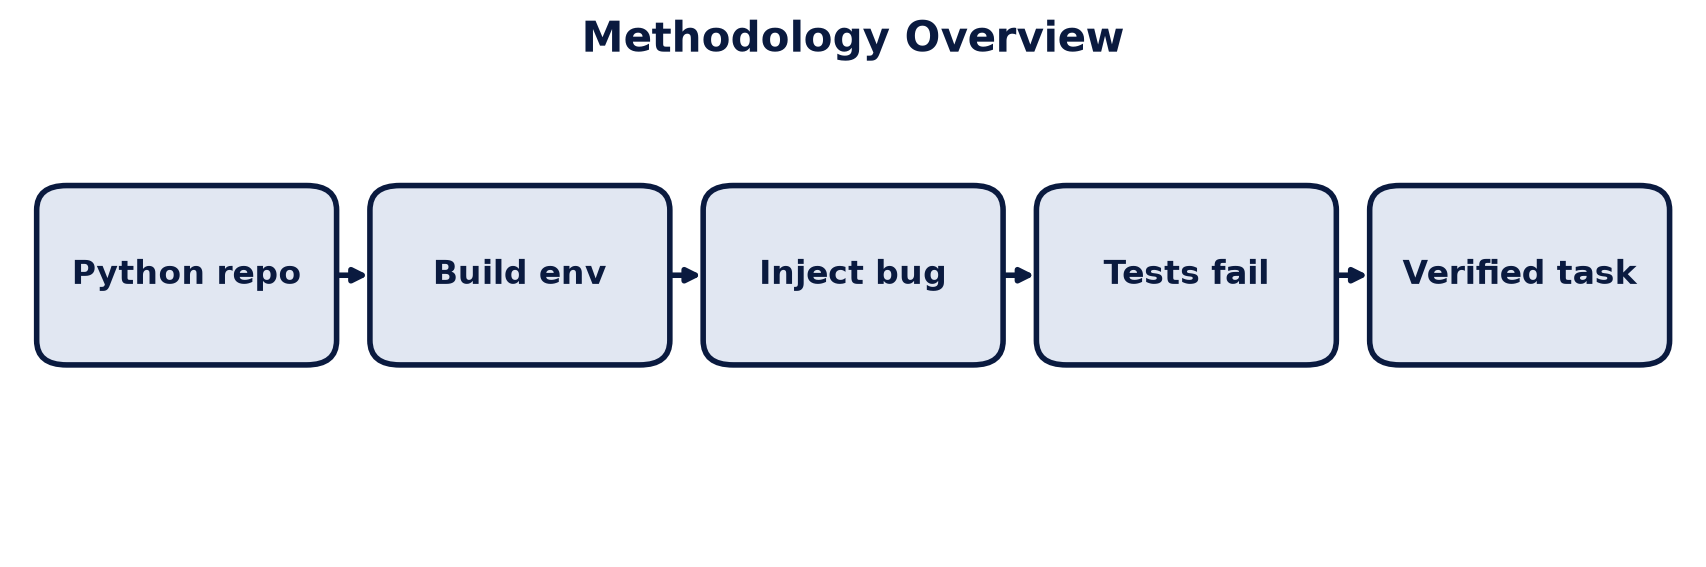
\includegraphics[width=0.9\textwidth,height=0.62\textheight,keepaspectratio]{images/swesmith_1.png}
\end{center}
\end{frame}

\section{System Architecture}
\begin{frame}{System Architecture}
\begin{center}
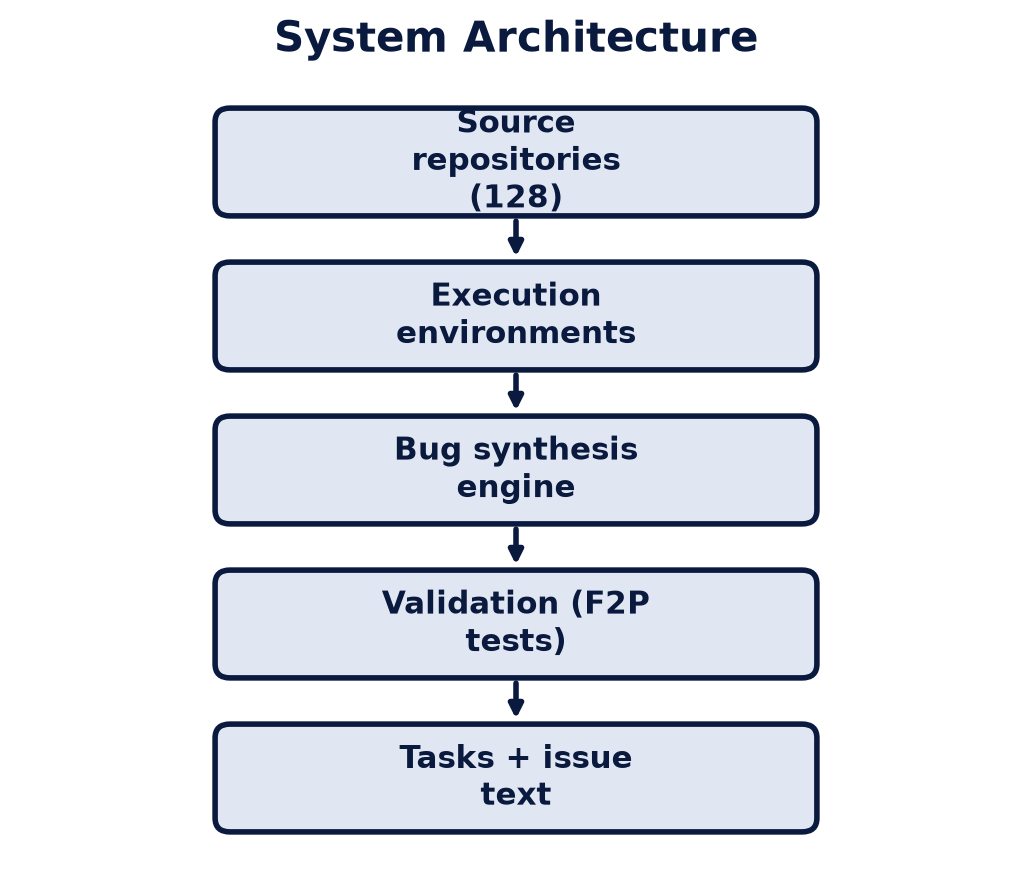
\includegraphics[width=0.9\textwidth,height=0.62\textheight,keepaspectratio]{images/swesmith_2.png}
\end{center}
\end{frame}

\section{Data Collection}
\begin{frame}{Four bug-generation strategies}
\begin{itemize}
\item LM Rewrite: rewrite from header and docstring.
\item LM Modify: inject errant edits into a function.
\item Procedural: AST edits, drop loop or flip operator.
\item PR Mirror: undo a merged pull request.
\item Combine patches for harder, multi-point bugs.
\end{itemize}
\end{frame}
\begin{frame}{Validation and scale}
\begin{itemize}
\item Keep patches that break passing tests (F2P).
\item Untouched code is the self-labeled fix.
\item LM drafts the issue from diff and failing test.
\item About 50{,}000 instances from 128 repos.
\item Only $\sim$295 GB, roughly 500x less storage.
\end{itemize}
\end{frame}

\section{Model Development}
\begin{frame}{Training SWE-agent-LM-32B}
\begin{itemize}
\item Base: Qwen2.5-Coder-32B-Instruct.
\item Run SWE-agent driven by Claude 3.7 Sonnet.
\item Rejection-sampling fine-tuning on successes.
\item 5{,}016 expert trajectories, 8{,}686 tasks.
\item Yields the open SWE-agent-LM-32B agent.
\end{itemize}
\end{frame}

\section{Results}
\begin{frame}{Resolve rate on SWE-bench Verified}
\begin{center}
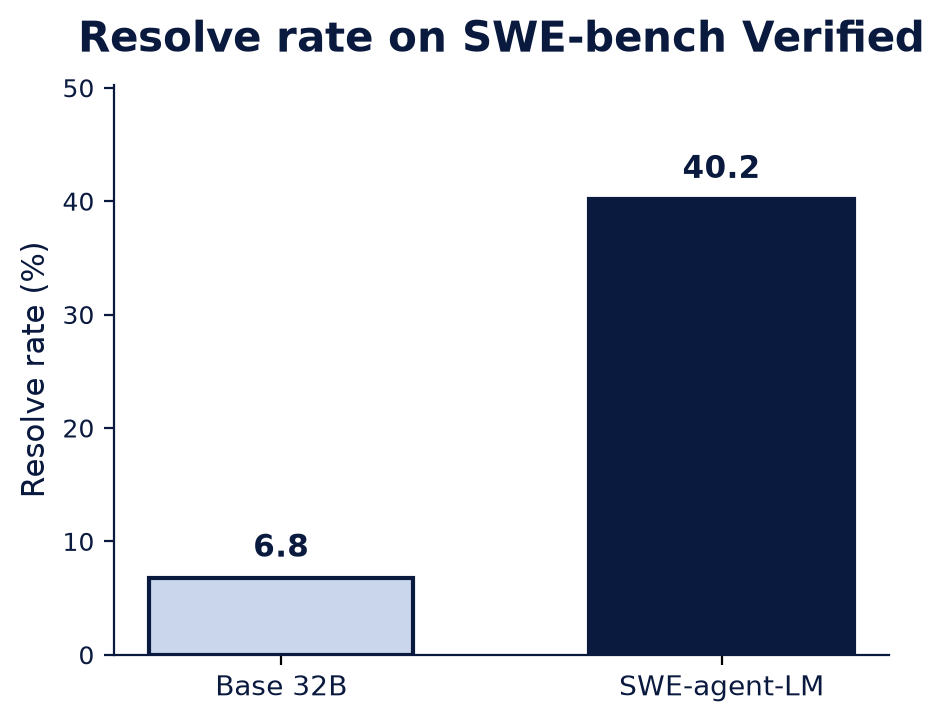
\includegraphics[width=0.9\textwidth,height=0.62\textheight,keepaspectratio]{images/swesmith_3.png}
\end{center}
\end{frame}
\begin{frame}{Key numbers}
\begin{itemize}
\item 40.2\% Pass@1 on SWE-bench Verified.
\item About +33.4\% over the base model.
\item State of the art among open-weight models.
\item Single attempt, no inference-time scaling.
\item 7B variant: 15.2\% Verified, 11.7\% Lite.
\end{itemize}
\end{frame}

\section{Discussions}
\begin{frame}{Why it works}
\begin{itemize}
\item Synthetic bugs give a reliable pass/fail signal.
\item Self-labeling removes manual annotation.
\item Multiple strategies broaden bug diversity.
\item Cheap storage unlocks order-of-magnitude scale.
\item Fine-tuning transfers to real GitHub issues.
\end{itemize}
\end{frame}

\section{Challenges}
\begin{frame}{Limitations}
\begin{itemize}
\item Pipeline is Python-centric.
\item Synthetic bugs may differ from real ones.
\item Only fine-tuning shown, no reinforcement learning.
\item Environment build is still per-repo effort.
\end{itemize}
\end{frame}

\section{Future Work}
\begin{frame}{Directions}
\begin{itemize}
\item Extend the pipeline to other languages.
\item Explore reinforcement learning on the tasks.
\item Generate harder multi-file, multi-bug instances.
\item Broaden repository and domain coverage.
\end{itemize}
\end{frame}

\section{Conclusion}
\begin{frame}{Conclusion}
\begin{itemize}
\item SWE-smith scales SE agent data automatically.
\item Verifiable bug-fix tasks from any Python repo.
\item 50{,}000 instances, 128 repos, low storage.
\item SWE-agent-LM-32B: 40.2\%, open-model SOTA.
\item Data, models, and trajectories are open-sourced.
\end{itemize}
\end{frame}

\section{References}
\begin{frame}{References}
\footnotesize
\begin{itemize}
\item J. Yang, K. Lieret, C. E. Jimenez, \emph{et al.}, ``SWE-smith: Scaling Data for Software Engineering Agents,'' arXiv:2504.21798, 2025.
\item C. E. Jimenez, J. Yang, A. Wettig, \emph{et al.}, ``SWE-bench: Can Language Models Resolve Real-World GitHub Issues?,'' in Proc. ICLR, 2024.
\item J. Yang, C. E. Jimenez, A. Wettig, \emph{et al.}, ``SWE-agent: Agent-Computer Interfaces Enable Automated Software Engineering,'' in Proc. NeurIPS, 2024.
\end{itemize}
\end{frame}
\begin{frame}\vfill\centering{\Huge Thank You}\vfill\end{frame}
\end{document}
